\chapter{绪论}
\label{cha:intro}

\section{引言}

自万维网创始人Time Berner-Lee于1998年提出语义万维网的概念\cite{berners1998semantic},语义网的发展逐渐受到业界人士的广泛关注。语义万维网是万维网的扩展,其数据应带有一定的语义信息,使得计算机可自动理解并处理各数据直接的联系,从而促进人类与计算机之间的相互合作。不同于用HTML显示实现人与人共享信息的万维网发展第一阶段,第二阶段,即语义网的建立,需要对现有的Web内容进行分析,标记,使其带有机器可以阅读的语义信息。由于传统的HTML文本只是从页面显示的角度进行了规范,没有在内容理解上进行预处理,这就决定着万维网向语义网的转变并不是一帆风顺。如何处理万维网的海量数据,以一种可理解的语义形式将其重新呈现,是当前语义网领域的研究热点之一。

为了实现语义万维网的远景,万维网联盟(W3C)于2007年2月提出Linked Open Data概念,并于之后启动了LOD项目,旨在为开放的语义数据集提供规范统一的组织规则。已有数据集都以URIs、RDF的形式公开在网上,并利用RDF链接关联不同数据源中的相关元素~\cite{bizer2009linked}。根据LOD cloud diagram\footnote{http://lod-cloud.net/} 网页上显示,截止到2014年8月的最新统计,LOD项目已发布了xxx个数据集,共含有xxx个RDF三元组。万维网上发布的链接数据,为语义网数据规范提供了示例,是计算机处理语义的基础,他们推动着知识的共享,对语义网的发展起着举足轻重的作用。相信随着LOD项目的推广,语义网影响的传播,还会有更多来自不同领域,基于不同语言的数据集发布出来。

在LOD项目中,有一些广为人知的开放数据集,如跨领域的YAGO\cite{suchanek2007yago,suchanek2008yago,hoffart2013yago2,mahdisoltani2014yago3},DBpedia\cite{auer2007dbpedia,bizer2009dbpedia,lehmann2015dbpedia},FreeBase \cite{bollacker2008freebase},Wikidata\cite{vrandevcic2014wikidata,erxleben2014introducing},限定领域的如电影领域的LinkedMDB\cite{hassanzadeh2009linked}与学术领域下的DBLP。这些数据集融合了从网页等数据源中的信息,将其机构化、标准化,便于查询与数据链接。然而,在语义万维网与链接数据蓬勃发展的同时,中文知识依然匮乏。DBpedia基于维基百科构建,横跨包括电影、人物、地理等在内的多个领域,生成了xx个三元组,有囊括英语、德语、法语、日语等xxx个语言版本,它因数据量众多、涉及内容广泛、结构较为完善,被视为链接数据的中心,然而DBpedia还不包含简体中文知识。另一个广受关注的知识库YAGO,在第三版本YAGO3中通过维基百科加入了德语、法语、意大利语等多国语言信息,但依然没有中文知识在其中。Wikidata由维基媒体基金会支持,完全基于维基百科源数据建立,含有一定数量的中文数据,但其中文知识数量受限于维基百科,图\ref{fig:wiki-stat}, 显示截止到2016年3月维基百科中几个主要语言的词条数量,当前中文词条仅有xx万,仅为英文词条xxx万的十分之一。由此可见,单纯基于维基百科建立知识库,在知识量上会受百科原有数据的限制,而中国用户在维基百科的参与度不高,中文知识的匮乏直接导致中文知识库创建困难,中文资源问题亟待解决。

\begin{figure}[H] % use float package if you want it here
  \centering
  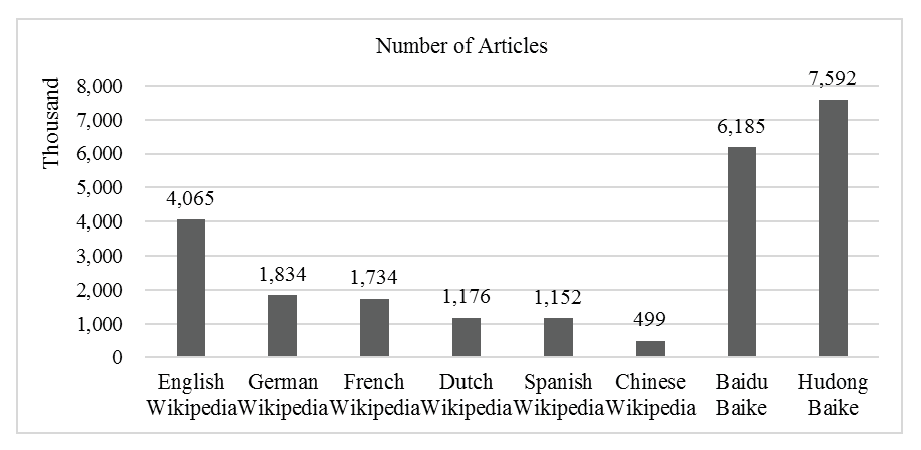
\includegraphics[width=0.8\columnwidth]{fig_stat}
  \caption{几个主要百科词条数量分布情况}
  \label{fig:wiki-stat}
\end{figure}

事实上,国内存在一些知名的通用领域的商业化百科全书,如百度百科\footnote{http://baike.baidu.com/}与互动百科\footnote{http://www.baike.com/},这些在线百科经过数以万计的人员撰写修改,已经形成很大规模,并存有丰富的中文知识。如果能融合两个中文百科的信息,平衡中英文知识量级就可能实现。

国内切实存在一些商业化的中文知识库,如搜狗“知立方”和百度“知心”,它们都是以人性化搜索、个性化推荐为出发点所建立的知识图谱产品。研究领域也有Zhishi.me\cite{niu2011zhishi} 等中文知识库。然而,随着开放链接的增多,人们发现单语言数据集已经不能满足语义万维网知识融合,知识共享的特点。YAGO向多语言知识库的进化,也说明跨语言的知识库有着更广泛的应用价值。除了更好的融合多语言知识,跨语言链接还用来辅助机器翻译[引用]、跨语言信息检索[引用]等。然而因为维基中文知识匮乏,中英文难以对齐等原因,中英文的跨语言链接还很少,也没有成形的已对齐的中英文知识库。

基于上述两个问题,本文对跨语言知识库的构建进行了探究,并融合多个在线百科丰富的知识,形成了中英文双语的大规模知识库,为中英文知识共享打下了基础。

在跨语言知识库构建过程中,如何获取更多的跨语言链接,如何对齐不同语言的本体,是主要关注的研究点。本体相当于一个知识库的骨架,是xxxx。通常本体包含概念与属性,概念是对一些相似事物抽象出的类别,属性为这些相似事物共有的特性。在RDF的定义中,有一些已定义的核心属性,如Rdf:type建立了实例与概念的instanceOf关系,也可以自定义属性。基于百科构建的知识库,通常以词条中的信息框属性作为该词条实例的自有属性,由此设定的自定义属性可达上万个。在跨语言知识库的构建过程中,我们要对概念下的属性集合有所筛选,也需要对这些自定义属性进行跨语言分析。属性的分析,对准确地描述本体、构建知识库起着重要作用。如果两种数据源的属性集合与属性值不一致,对不同语言的知识查漏补缺、修正错误,也有着积极的意义。基于知识库中属性的重要性,本文我们对百科的信息框属性进行了领域模板分析与对齐,力求获得更准确的本体框架,以及发现更多的跨语言链接。


\section{主要工作}
本节对文章涉及的主要工作进行初步的描述:以解决中文知识匮乏,提高中英文信息的融合度,进而实现知识共享为目的,我们构建了一个通用领域的跨语言的知识库。在构建过程中,面临schema的归一化与对齐问题,本文重点聚焦到属性对齐这一研究方向上。本章对涉及到的研究点进行了概括,并提出可能遇到挑战。

\subsection{基于百科模板的跨语言属性对齐}
不同于大多数的跨语言属性对齐研究,本文对属性的研究同时含有跨异构百科的特性,即为服务于随后的基于多个百科源构建知识库的任务,本文对属性的研究建立在维基百科与百度百科两个异构百科上,结构与语言的双重障碍,为属性对齐的研究增加了难度。为尽可能达到结构上的统一,我们引入领域模板概念,并将属性对齐问题限定在领域范围下,同时利用中文维基为英文维基与百度百科搭桥引线,获取更多关联信息。总结来说,该问题通过四个步骤解决并优化,分别为:1)获取中英文属性对齐种子集合, 2)生成百科领域模板,3)同语言相似属性合并, 4)跨语言属性对齐。图xx展示了该方法的框架图。

{\heiti 问题定义:} 给定两个中英文异构百科$W_{e}$与$W_{z}$,在限定领域$D$下,获得该属性集合,生成领域模板${T_{D}}$,并在该模板下,聚集相似属性组成超级属性$sp$,对齐跨语言属性$sp_{e} \Leftrightarrow sp_{z}$。

{\heiti 面临挑战:} 本项工作面对跨百科与跨语言两重困难,可能面临如下挑战:1)异构百科存在的编辑规则不一致,使得即使是相同语言也存在对齐问题,如何尽可能抽取更多的对齐关系?2)领域界限模糊不清,如何构建认可度高的领域模板? 3。。。


\subsection{中英文跨语言知识库的构建}
本文提及的知识库系统XLore,其构建初衷是为解决中文知识匮乏问题,提高知识融合度与共享率,面对当前多语言在线百科与知识库中中英文信息极度不平衡的现状,利用其他丰富的中文资源不失为一则良策。基于此我们将目光聚焦在国内信息最丰富的两大在线百科全书——百度百科与互动百科上,利用两大百科的词条页面信息、分类体系数据,并结合维基百科对外发布的数据存储文件,抽取结构化信息,经过一系列的知识处理流程,获得语义信息,构成跨语言知识库XLore。图xx为XLore的构建框架。

值得一提的是,我们对XLore知识库的应用层次上也进行了尝试,主要体现在支持数据访问的在线系统以及提供实体语义信息的API接口。

{\heiti 问题定义:} 我们将在线百科定位为$W$, 一个$W$中包含知识库构建所需的重要信息,比如分类系统与词条页面,知识库将筛选并融合这些信息,它是一系列实体、概念等形式化集合。

如果将知识库(Knowledge Base)定义为$KB$,则
跨语言知识库({\heiti C}ross-{\heiti L}ingual {\heiti K}owledge {\heiti B}ase)的工作则定义为:$CLKB = <KB_{z}, KB_{e}>$, 其中$KB_{z}$ 与 $KB_{e}$分别为中、英文知识库。而构建跨语言知识库的工作,则是从多个中英文百科资源中集合知识构建$CLKB$。

{\heiti 面临挑战:} 本项工作的主要挑战包含:1)如果从百科中定义知识库中的三大元素:概念、属性、实体? 2)如何解决跨语言面临的基本问题——获取更多的跨语言链接?3)如何优化本体schema,避免杂乱的百科数据引入的杂质?


\section{主要贡献}
本文提出了一种领域模板生成与领域跨语言属性对齐的方法,并利用对齐结果与四个百科数据源的抽取结果,构建通用领域的中英文知识库XLore,其中主要贡献列举如下:
\begin{itemize}
\item {\heiti 1) 领域模板下的跨百科跨语言属性对齐,} 工程抽取与算法计算相结合,提取出英文维基百科与百度百科两个异构百科下的信息框属性关系。包括百科下属性模板生成,与限定领域下的中英文属性匹配。该方法在构建大规模知识库过程中,对于从多语言的异构数据源生成对齐的shema有一定的贡献。
\item {\heiti 2) 构建了通用领域的跨语言知识库XLore,} 融合基于不同语言的异构百科,获取语义信息,解决中英文知识数量不平衡的问题,该知识库是当前大规模的中英文知识库之一,在跨语言语义网络上有着无限的应用潜能。
\item {\heiti 3) 提供了便于数据访问的可视化系统与应用接口,}前者分别从一般用户与专业用户的不同角度,给出搜索框查询与SPARQL查询两种知识访问方式;后者考虑知识库的应用场景,提供基于RestFul的实体访问API,对给定文本进行实体分析与排歧,返回实体语义信息,实现了一定应用价值。
\end{itemize}

\section{论文组织}

本文通过绪论、研究现状、基于百科模板的跨语言属性对齐、大规模中英文跨语言知识库XLore的构建、XLore系统与应用接口、总结与展望共6个章节来组织全文内容,其章节关系与结构组织如图\ref{fig:organization}所示:

\begin{figure}[H] % use float package if you want it here
  \centering
  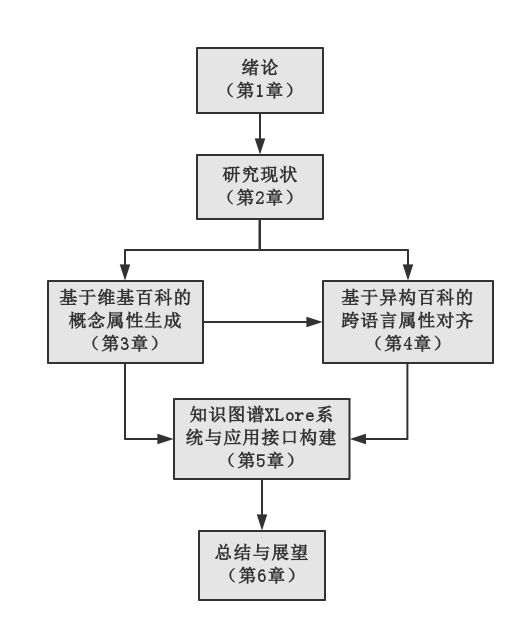
\includegraphics[width=0.5\columnwidth]{organization}
  \caption{论文组织结构图}
  \label{fig:organization}
\end{figure}

第 1 章为绪论,对本文的研究背景进行描述,概要地介绍工作内容,并交待论文的主要贡献及文章组织结构;

第 2 章为研究现状,对当前构建跨语言知识图谱过程的跨语言对齐研究现状进行描述,包括实例对齐、属性对齐,此外列举当前广为人知多语言知识图谱与中文知识图谱,并介绍其构建技术;

第 3 章描述了基于百科模板的跨语言属性对齐流程。首先通过观察与抽取百科中的模板与属性,获得初始的属性集合,之后进行领域模板生成的分析,并实现在特定领域下,同语言相似属性的对齐与跨语言属性链接;

第 4 章介绍了基于在线百科,构建跨语言知识图谱的过程。该工作从中英文维基百科、百度百科、互动百科中抽取语义数据与跨语言关系,并复用第3章的研究结果,对齐中英文知识,致力于解决中英文知识不平衡问题;

第 5 章介绍了基于第4章构建的知识库而搭建的可视化系统与数据访问接口,从实际应用角度展示XLore知识库的结构化与可用性;

第 6 章对本文提出的跨语言属性对齐与知识图谱构造研究工作进行了总结和展望,分析了不足之处,为下一步研究提出了新的建议和意见。
 

